\section{Was ist Bisphenol-A?}
\subsection{Entstehung und Anfangszweck}
Die britischen Biochemiker Edward Charles Dodds und Wilfrid Lawson suchten
im Jahr 1936 nach Chemikalien, welche das natürliche Sexualhormon Östrogen in medizinischen
Therapien ersetzen kann, da dieses noch aus dem Urin von trächtigen Stuten
aufbereitet werden musste, was sehr kostenaufwendig war \cite[]{Umweltbundesamt2010}.
Wie man gegenwärtig jedoch sieht, ist Bisphenol-A kein Pharmazie-Produkt, da die selben Forscher
später weitaus bessere synthetische Östrogene entdeckten, weshalb Bisphenol-A im Bereich
der Hormontherapie ausfiel \cite{Wikipedia}.
\subsection{Hormonelle Wirkung im humanen Körper}
Stoffe, welche wenn sie ab einer bestimmten Konzentration in ein Hormonsystem gelangen,
dieses verändern und somit die Entwicklung der Embryonen stören bzw. die Fortpflanzung
beeinflussen, werden \textit{Endokrine Disruptoren} genannt.
Durch das Andocken, der Stoffe an die für eigentlich natürlichen Sexualhormone
vorgesehenen Rezeptoren, werden diese entweder aktiviert oder gehemmt \cite{Umweltbundesamt2010}.
Bisphenol-A zeigt Untersuchungen zufolge, dass weibliche Sexualhormone gestärkt werden und
gleichzeitig männliche Sexualhormone gehemmt werden.
Im humanen Körper wird Bisphenol-A zwar sehr schnell zu Bisphenol-A-Glucuronid und
Bisphenol-A-Sulfat metabolisiert und somit unschädlich gemacht, allerdings
können in menschlichen Zellgeweben wie Hoden und Mutterkuchen die unmetabolisierte wirksame
Form (auch freie Form genannt) freigesetzt werden \cite{Umweltbundesamt2010}.
Diese Freisetzung führt vor allem zu einer zunehmenden Unfruchtbarkeit bei Männern. Nach Auswertungen zufolge liefern die UBA und NGO CHEM Trust Studien, wurde bei Probanden die einen erhöhten Bisphenol-A-Spiegel im Blut hatten, einen Zusammenhang mit Diabetes,Fettleibigkeit, Herz-Kreislaufproblemen und einer fehlenden Libido(Sexual-Triebe) festgestellt.
\subsection{Chemische Darstellung}
Bisphenole werden durch die Reaktion von Phenolen mit Carbonylverbindungen(Kohlenstoffatome, welche ein doppelt gebundenes Sauerstoffatom tragen) erhalten. Bisphenol-A entsteht also durch die Reaktion von Phenol mit Aceton (Deshalb das \glqq A\grqq{} in Bisphenol-A). Dargestellt, wird es durch 2 Äquivalenten Phenol und einem Äquivalent Aceton(Abbildung 1.). Um eine höhere Ausbeute zu erhalten, wird mit einem Überschuss an Phenol gearbeitet \cite{Herstellung}. Die Summenformel ist: \ce{C15H16O2}.\\
\begin{figure}[htpb]
    \centering
    
\includegraphics[width=.75\textwidth]{Darstellung.png}
    \caption{Darstellung \cite{Wikipedia}}
\end{figure}
\newpage
\subsubsection{Zwischenschritte bis zum Endprodukt}
Hierbei ist von einer elektrophilen aromatischen Reaktion die Rede. Aufgrund des elektrophilen \glqq Angriffs\grqq{} vom Formaldehyd gerät man zunächst zum Sigma-Komplex. Die folgenden Abbildungen sind alle selbsterstellt.
\begin{figure}[htpb]
    \centering
    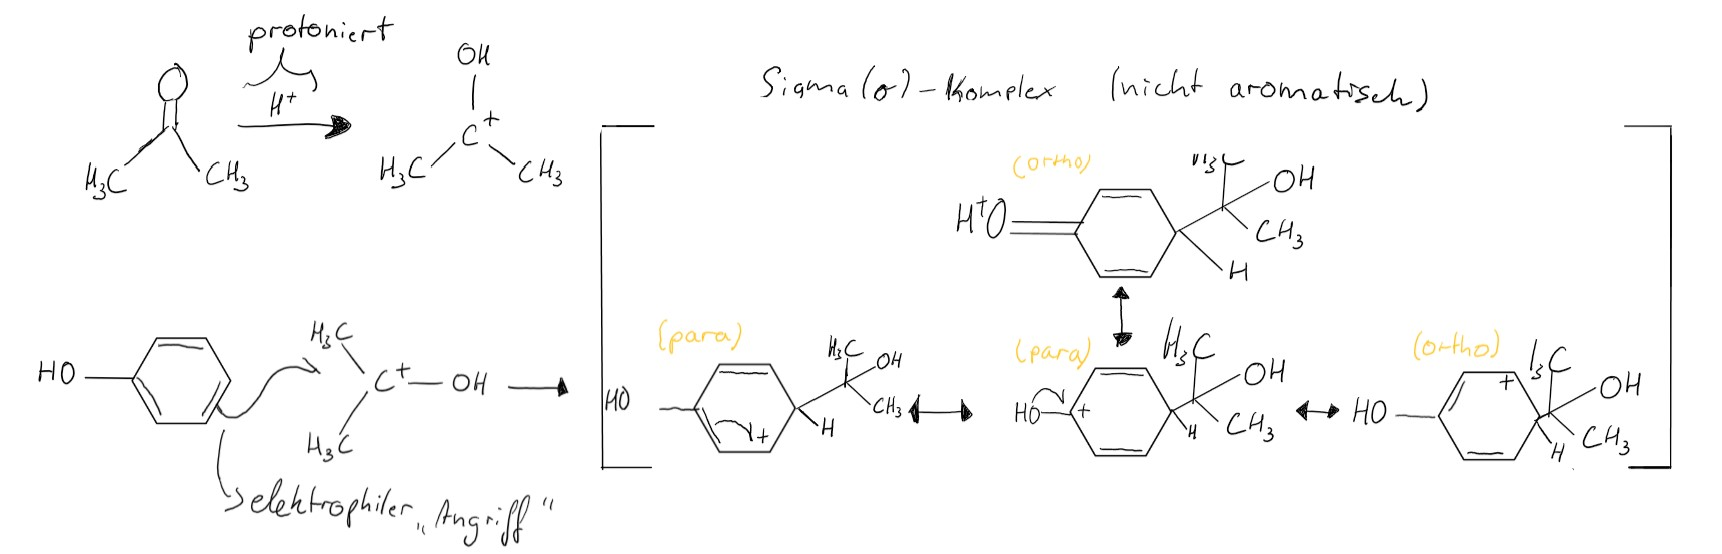
\includegraphics[width=.75\textwidth]{Sigma.jpg}
    \caption{Sigma-Komplex}
\end{figure}
\\Die Hydroxyd(OH)-Gruppe gehört zu den Substituenten mit +M-Effekt, dieser beeinflusst stark die \glqq Aktivierung\grqq{} der aromatischen Verbindung. Die OH-Gruppe spielt die Rolle des Dirigenten und dirigiert die Zweitsubstituenten in die para- und ortho-Stellungen. Wie man zu erkennen mag, lassen sich also dadurch vier Grenzstrukturformeln formulieren, davon jeweils zwei para-und ortho-Grenzstrukturformeln. Aufgrund der sterischen Hinderung wird nur das para-Produkt gebildet. Da der Sigma-Komplex nicht aromatisch ist, reagiert dieser durch Abspaltung eines Proton ab und es entsteht das Zwischen-Produkt 4-(2-Hydroxy-2-propyl)phenol\cite{Herstellung}:
\begin{figure}[htpb]
    \centering
    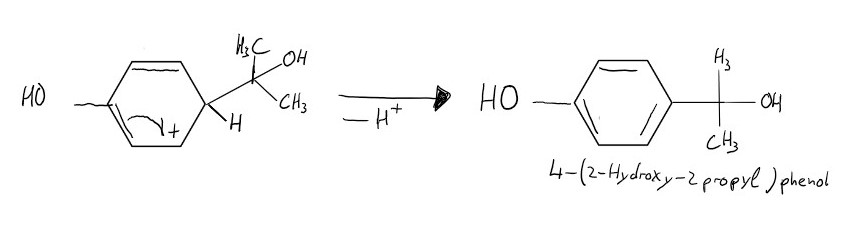
\includegraphics[width=.75\textwidth]{Zwischenprodukt.jpg}
    \caption{Zwischen-Produkt}
\end{figure}
\\Die OH-Gruppe vom erhaltenen Zwischen-Produkt wird nun protoniert und abgespalten, dies geschieht da es sich in einer \glqq benzylischen-Stellung\grqq{} befindet und die restliche Ladung somit erneut dank Mesomerie stabilisiert.
\begin{figure}[htpb]
    \centering
    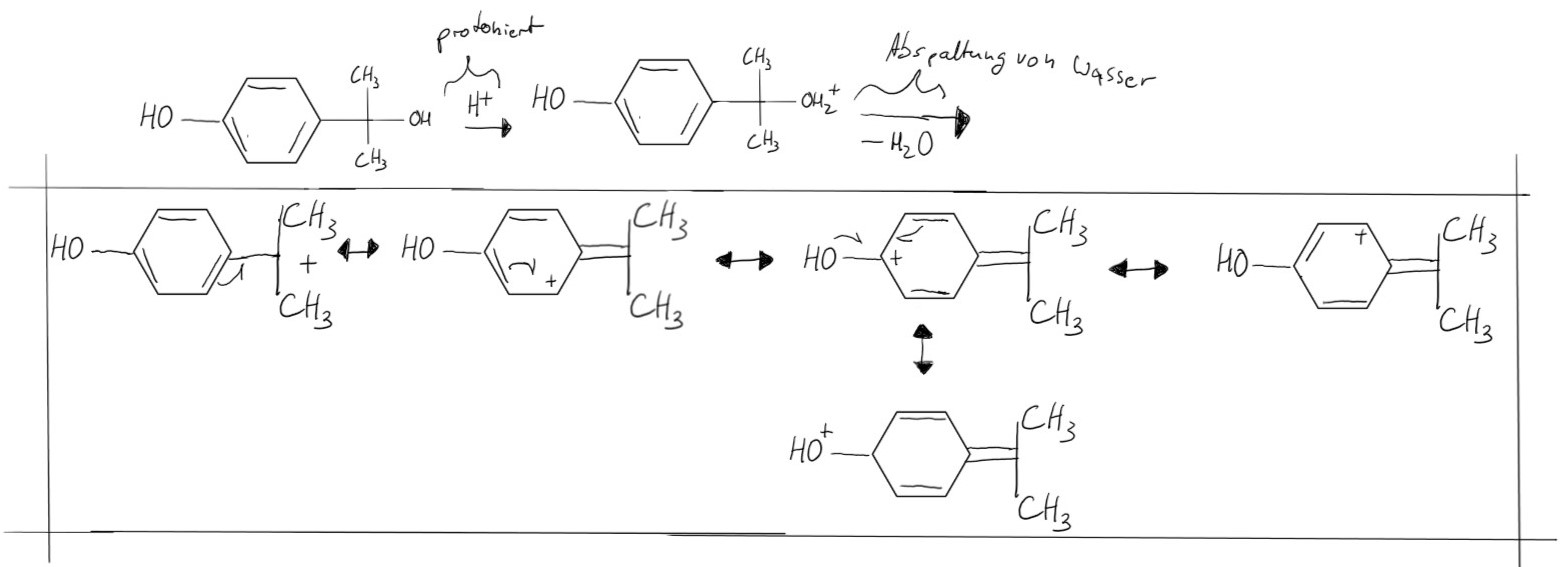
\includegraphics[width=.8\textwidth]{mesomerie.jpg}
    \caption{benzylische Stellung}
\end{figure}
\\Dadurch entsteht wieder ein Elektrophil, dieses greift in einer ähnlichen Reaktion das zweite Phenol-Molekül an und es entsteht Bisphenol A:
\begin{figure}[htpb]
    \centering
    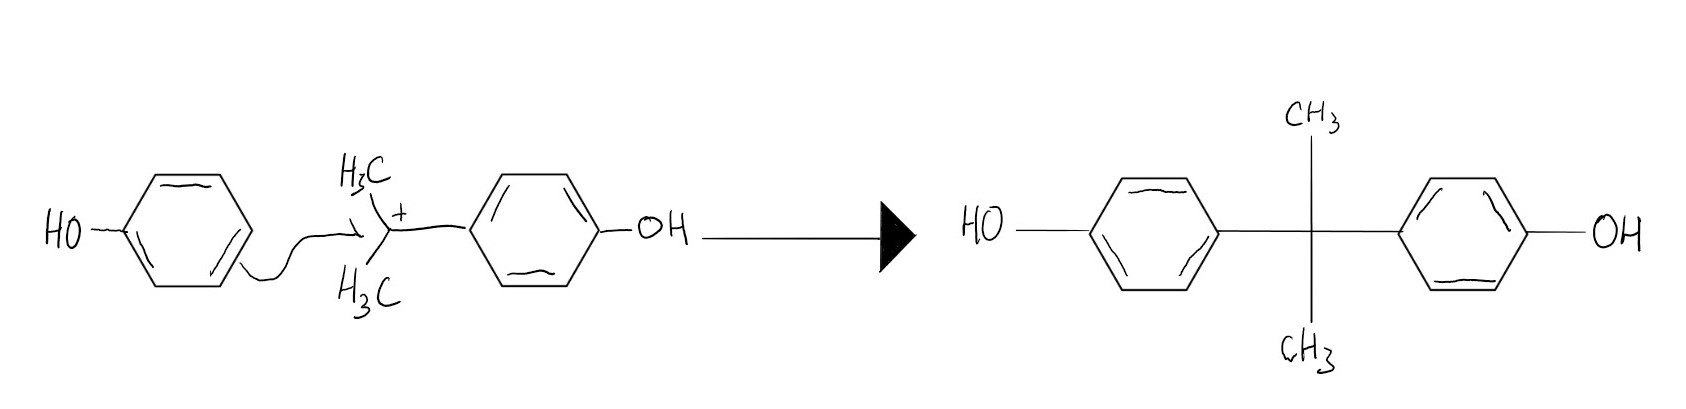
\includegraphics[width=1\textwidth]{BisphenolA.jpg}
    \caption{Bisphenol-A}
\end{figure}
\subsection{Hersteller}
Die weltweit größten Hersteller sind die US-Firmen \glqq Dow Chemical\grqq{} und \glqq Hexion Inc.\grqq{}, außerdem das taiwanesische Unternehmen \glqq Nan Ya Plastics\grqq{} sowie \glqq Ineos Phenol\grqq{} \cite{Wikipedia}.
\subsection{Freisetzung}
Die Freisetzung von Bisphenol-A erfolgt durch eine Hydrolyse der Esterverbindungen des Bisphenol-A Moleküls\cite{Freisetzung}. Bei der Hydrolyse werden die Esterverbindungen durch Reaktion mit Wasser gespalten. Diese wird durch Hitze, Säuren und Laugen beschleunigt. Ein gutes Beispiel dafür ist die Reinigung von Polycarbonat Produkten in der Spülmaschine, bei der das Wasser mit Reinigungsmittel gemischt und erhitzt wird, diese Umstände begünstigen natürlich die Freisetzung von Bisphenol-A in das Wasser und somit an jegliches anderes Geschirr. Außerdem kann auch eine Freisetzung nach mechanischen Schädigungen erfolgen, dies passiert beispielsweise bei der wiederholten, maschinellen Reinigung von Polycarbonat Flaschen.
